\subsection{Reference Implementation}

Before implementing a code generator one has to know what the target code is. Therefore a reference implementation has been
developed which was coded to large degree manually. From this reference code the templates can be derived. Also this is a
manual step.

We use a Java Server Faces (JSF) based application, which can be deployed on any Java Web Application server like Tomcat, JBoss etc.

The following screenshot shows the structure of the web application project. The application is available for download from the project 
homepage (\href{http://lwc13-xtext.eclipselabs.org.codespot.com/files/JSF-QL-1.0.zip}{JSF-QL-1.0.zip})

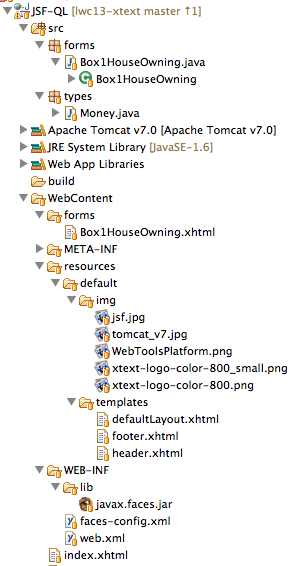
\includegraphics[width=10cm]{./images/chapter02/referenceimpl_projecttree.png}

Large parts of the application are not derivable from the model, they build the skeleton of the project. This is:
\begin{itemize}
\item Custom types (\texttt{src/types/*})
\item Custom type converter (\texttt{src/converter/*})
\item Images (\texttt{WebContent/resources/default/img/*})
\item Page Templates (\texttt{WebContent/resources/default/templates/*})
\item Libraries (\texttt{WebContent/WEB-INF/lib/*})
\item Web Application Descriptor (\texttt{WebContent/WEB-INF/web.xml})
\end{itemize}

We will focus on the parts which are dependent on the QL model and thus subject of code generation. These artifacts are:
\begin{itemize}
\item Java Bean classes representing the state of a Form (\texttt{src/forms})
\item JSF enabled XHTML pages representing the presentation of a Form (\texttt{WebContent/forms/*})
\item Index page (\texttt{WebContent/index.xhtml})
\item Faces configuration (\texttt{WebContent/WEB-INF/faces-config.xml})
\end{itemize}


